\subsection*{Punto 01}

\textbf{Ejecute cada inicialización 5 veces con diferentes semillas y muestre en una gráfica el mínimo y la media de la función obejtivo de k-medias como una función de k.}

En la figura \ref{fig:problema_04_mean_and_minimum} se muestra el promedio y mínimo de la función objetivo de inicializador del método de k-means. En esta se visualiza que la tendencia de las dos es semejante. La diferencia promedio entre la media y mínimo es 1.0729. Comparado con el orden de magnitud de la función de costo este valor es muy pequeño. Por lo que tomar el mínimo un promedio de los resultados no varia mucho en las predicciones de cada modelo.

\begin{figure}[H]
    \centering
    \begin{subfigure}{16cm}
        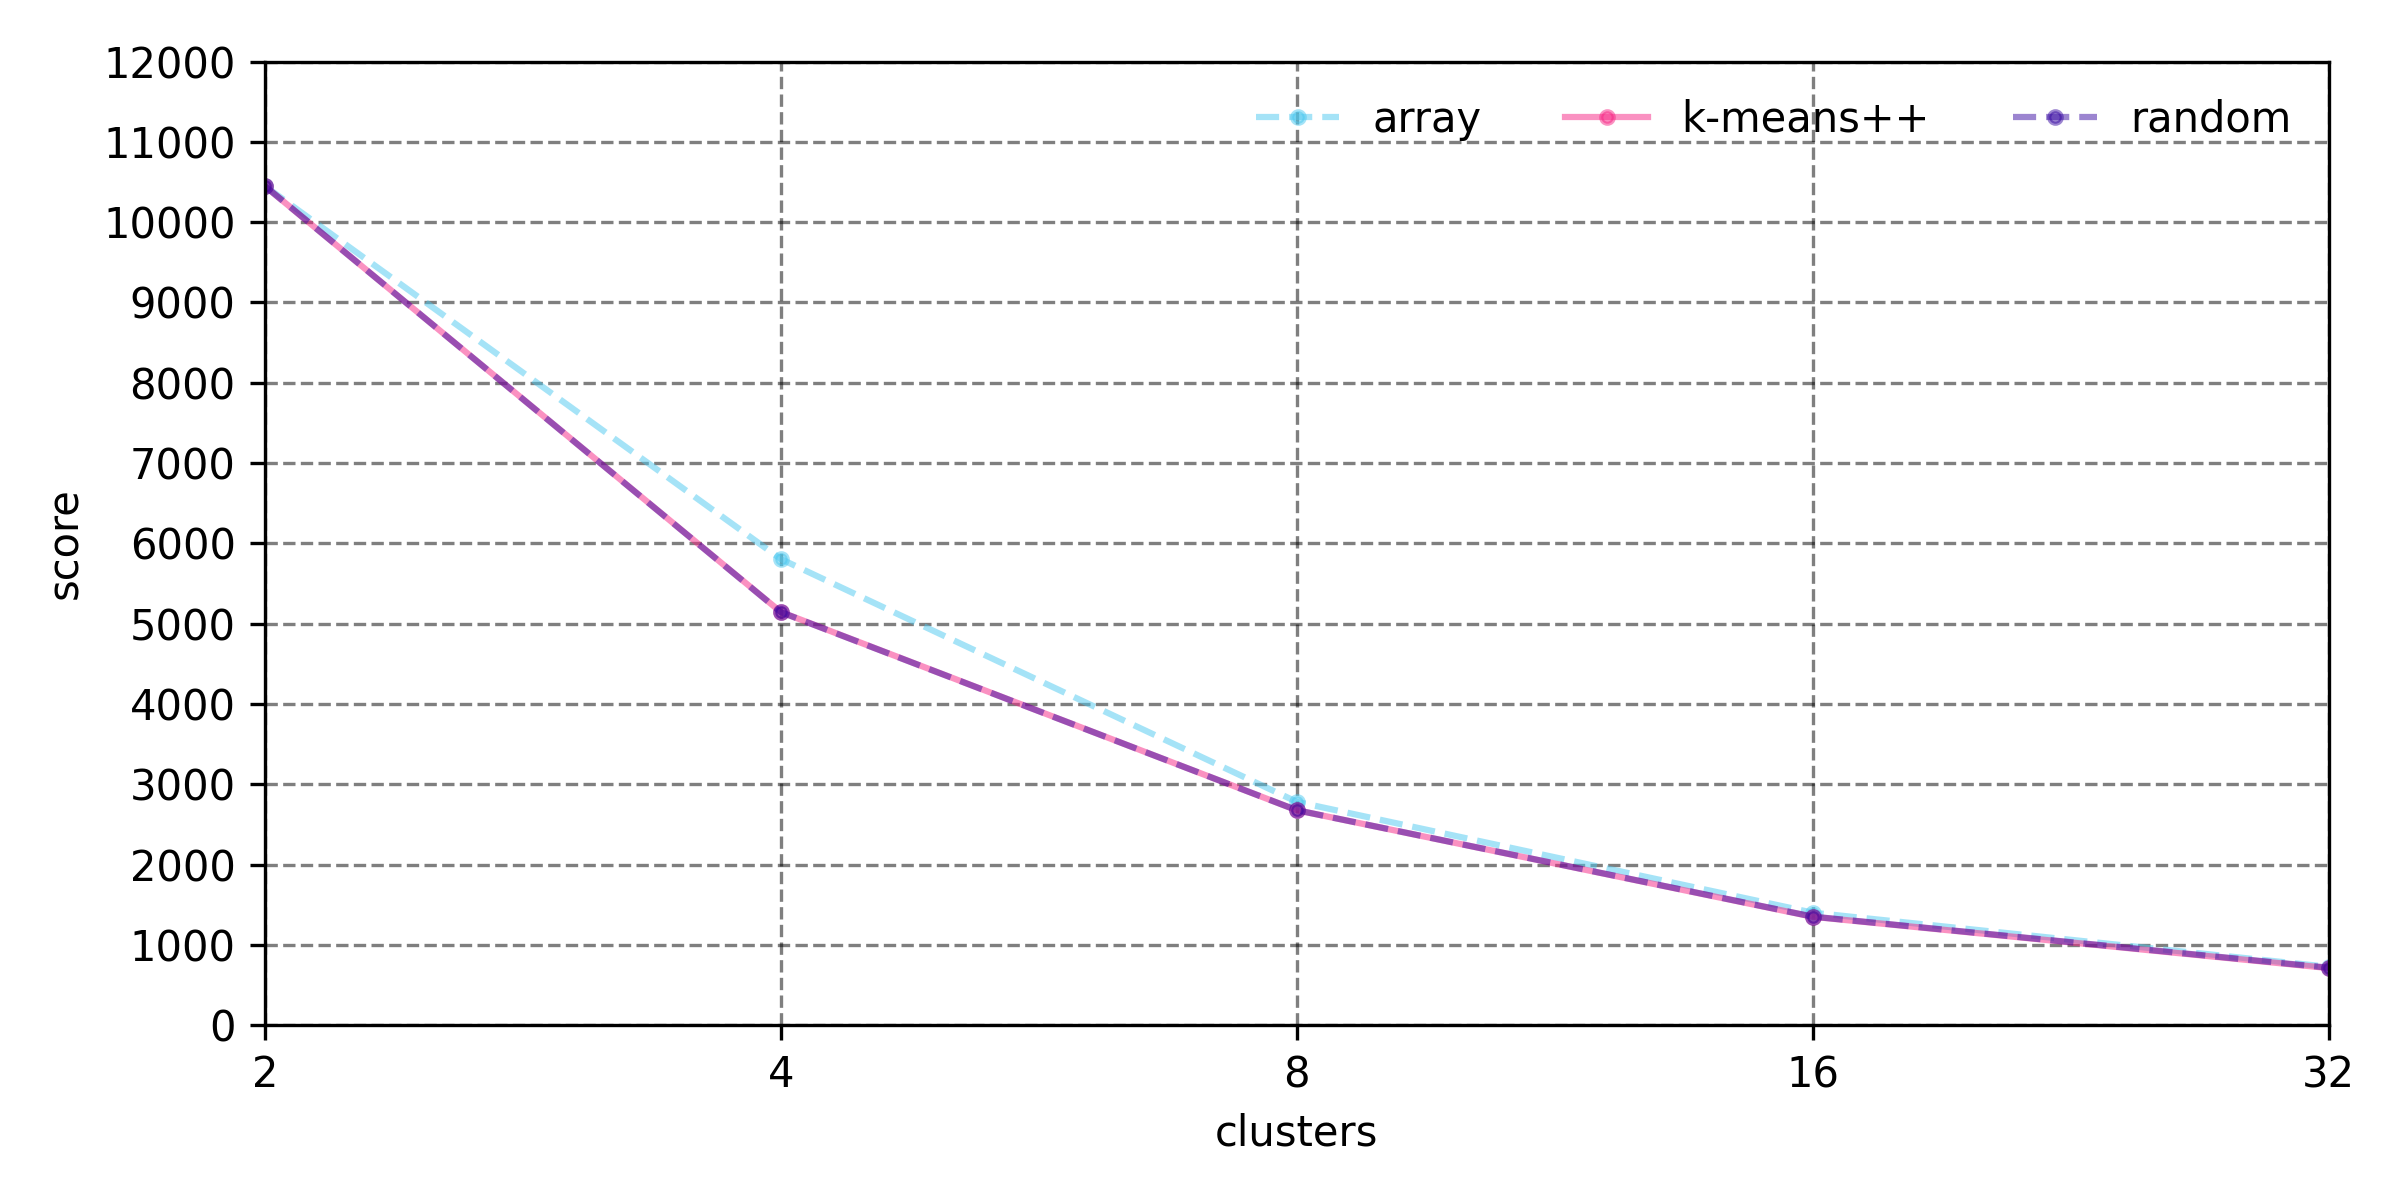
\includegraphics[width=16cm]{Graphics/Problema_04/mean_scores.png}
        \caption{Promedios de la función objetivo.}
    \end{subfigure}
    \begin{subfigure}{16cm}
        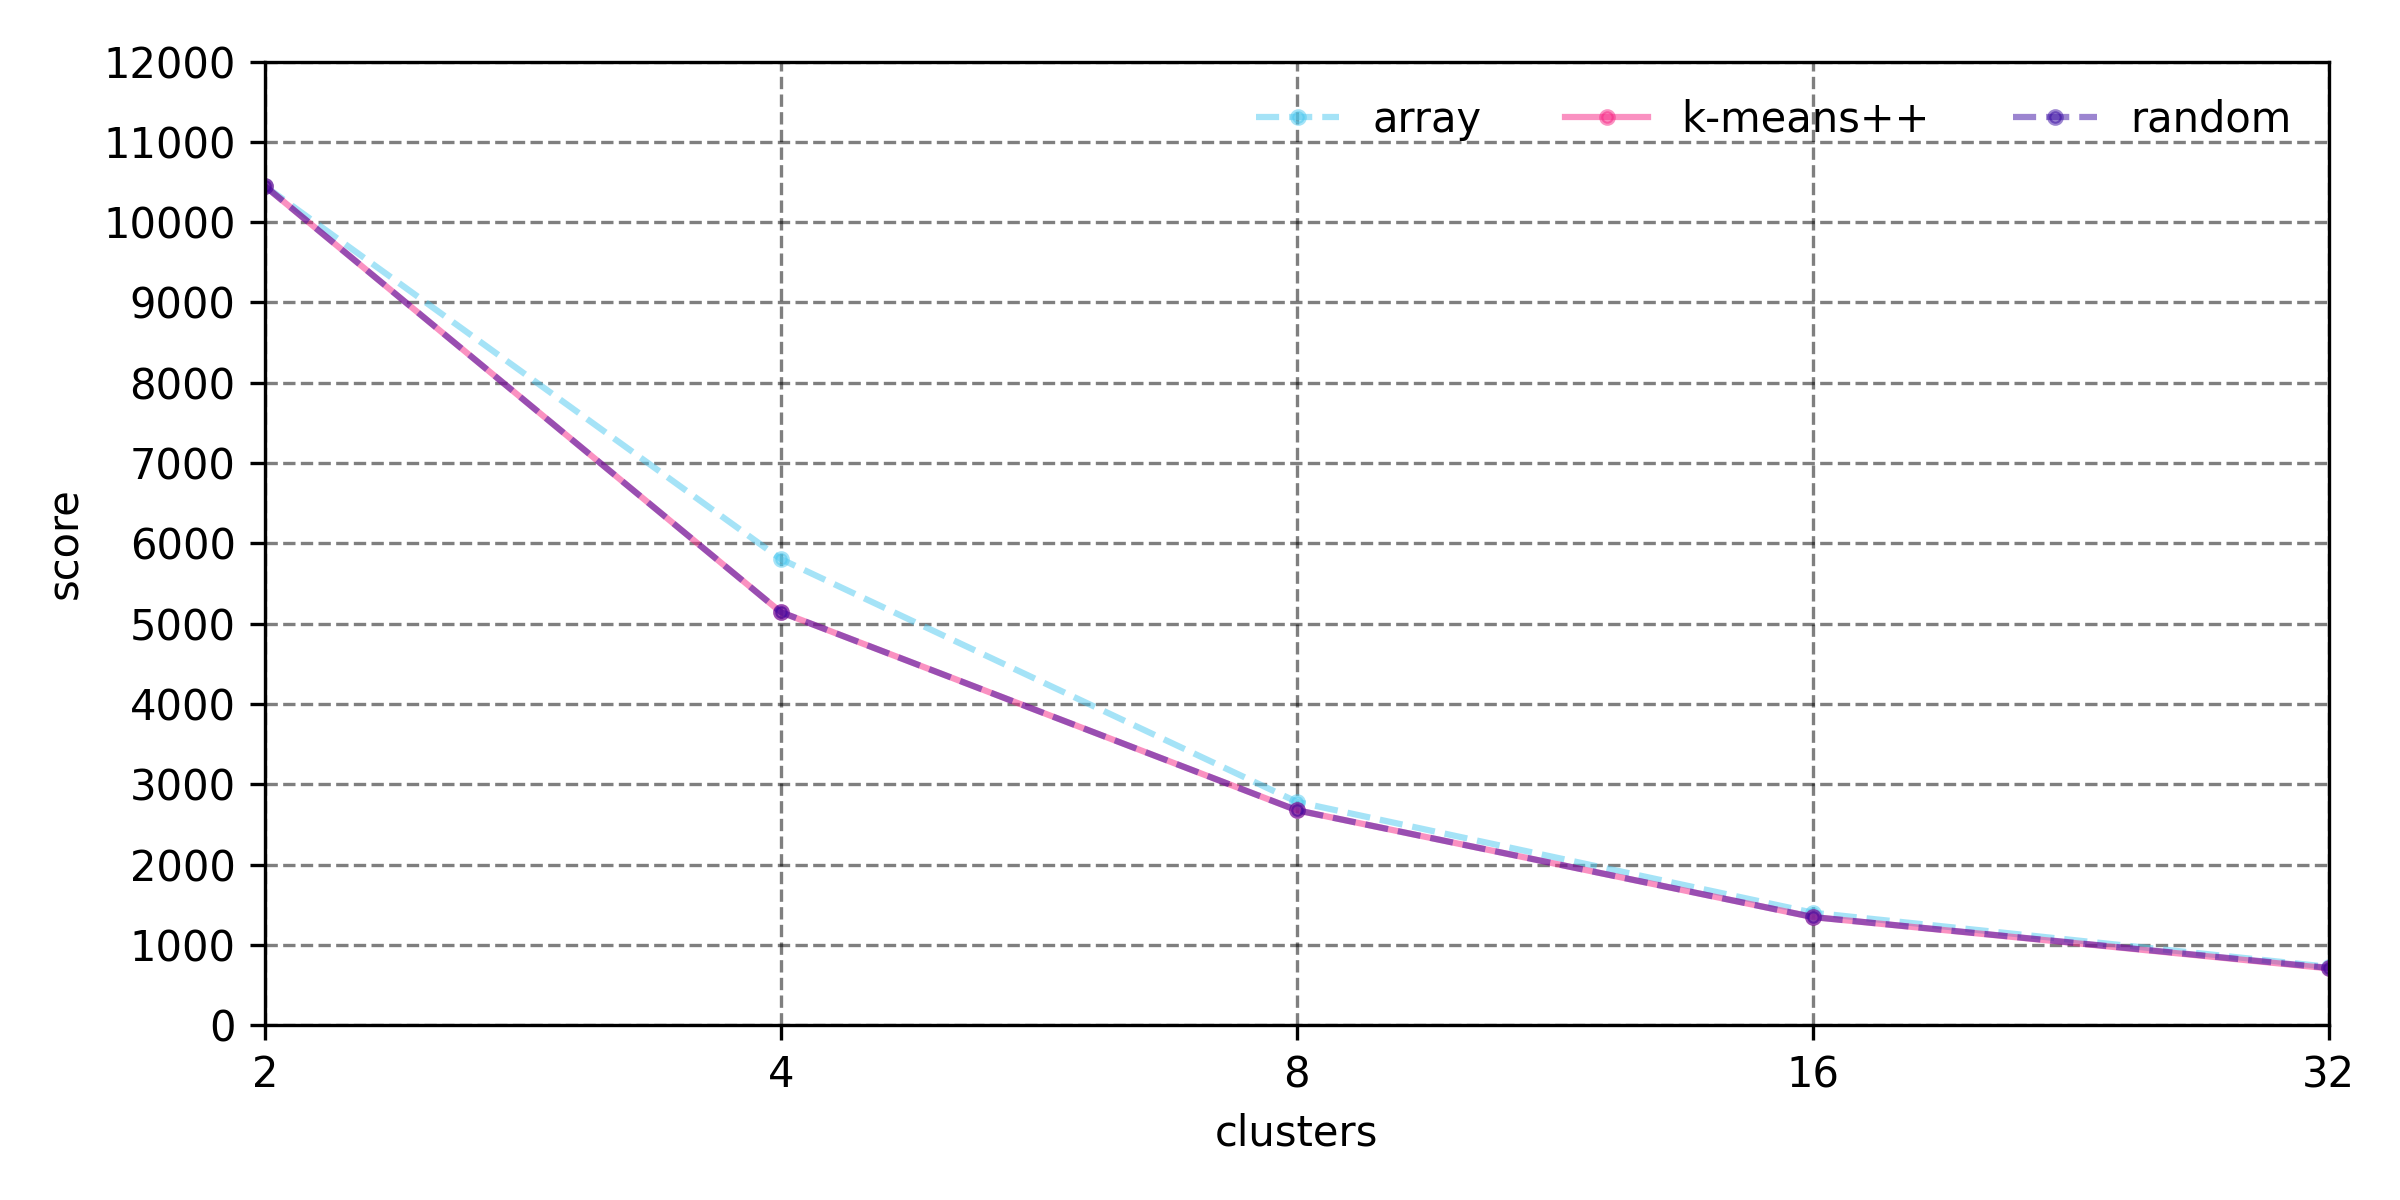
\includegraphics[width=16cm]{Graphics/Problema_04/minimum_scores.png}
        \caption{Mínimo de la función de objetivo.}
    \end{subfigure}
    \caption{Promedios y mínimo de la función objetivo de cada inicializador dado en el método de k-means.}
    \label{fig:problema_04_mean_and_minimum}
\end{figure}